\documentclass{report}
\usepackage{fullpage, graphicx} %Images and figures
\usepackage{rotating} %rotating images
\usepackage{titlepic} %Logo in title
\usepackage[margin=1in]{geometry} %margin control
\usepackage{hyperref} %hyperlinks
\usepackage{ulem} %strikethrough
\usepackage{color}
\usepackage{xcolor}
\usepackage[english]{babel}
\usepackage{tabularx,booktabs,ragged2e}
\newcolumntype{Y}{>{\RaggedRight\arraybackslash}X}
\usepackage{geometry} % set page block parameters suitably
\usepackage{etoolbox}
\usepackage{wrapfig}
\usepackage{float}


%In case we don't want page breaks for chapters
%\makeatletter
%\patchcmd{\chapter}{\if@openright\cleardoublepage\else\clearpage\fi}{}{}{}
%\makeatother



\title{\bf Cansat UK Progress Report 2}
\author{
	GWC Cansat\\
	George Watson's College	
}
\titlepic{\vspace{-20pt}
\includegraphics[width=8cm]{frontLogo}}
\date{December 2017}


\begin{document}
\maketitle
\tableofcontents
\pagenumbering{arabic}

\chapter{Progress Statement}
	%We need to shorten this chapter
	We have continued along our current plan, working on each 
	section of the project simultaneously in sub-teams. A summary 
	of our progress is shown below:

	\begin{description}
		\item[Team Administration] \hfill \begin{itemize}
			\item A member of our team has dropped out due to personal
			reasons. In order to maintain our forward momentum, we
			have taken on an additional member.
			\item We have recieved three new sponsorships; two have 
			provided us with extra funding surrounding our project,
			the third company providing us with free custom PCB 
			manufacturing.
			\item Having different sub-teams that have responsibilites for
			different	parts of the cansat development was leading to issues
			with team members not knowing how the overall	project was 
			progressing. The team leaders now collaborate to produce an
			internal report of progress every 2-3 weeks. This has recieved
			positive feedback within the team.
			\item We are continuing to maintain our website, hosted on the
			domain \url{gwccansat.com}, in addition to having officially launched our
			video blog (`vlog') programme, showing our progress on a weekly
			basis, leading up to the competition.
			\item The team has adopted new graphical designs for its logo and
			media/website backgrounds in order to give this year's campaign a fresh
			aesthetic.
		\end{itemize}
		
		\item[Mechanical development] \hfill \begin{itemize}
			\item We continue to work towards having a finalised 
			CAD model. This is dependent upon space requirements of
			our sensors and custom PCBs, so is still undergoing iterative
			revisions.
			\item Additionally, we are still working towards having a modular
			compartment for our secondary mission, allowing the cansat to
			be easily reused for other experiments with minimal physical
			changes made --- a simple case of plugging in and programming
			the new, relevant sensors.
		\end{itemize}

		\item[Electronics design] \hfill \begin{itemize}
			\item Our team hit some budgeting issues, leading us to
			consider other electronics options --- primarily in--house 
			assembly, as an alternative to PCB fabrication. This was recently
			resolved with the addition of our new sponsors, providing us
			with free PCB fabrication and more funding.
			\item We also now have an initial schematic design, that is 
			ready to be made into a PCB design, provided that the software
			team have successfully interfaced and tested all the sensors and
			the mechanical team have provided ideal locations for the larger
			components on the PCB.
		\end{itemize}

		\item[Software design] \hfill \begin{itemize}
			\item Currently, the project progress is fullcruming off the
			dependency on testing the sensors from our current design.
			Hence, we have allocated extra team members and 
			resources to this section.
			\item We are currently working on testing each individual sensor, 
			to ensure that we are able to interface with them correctly with
			the current wiring solution and ready to make notes of any required 
			amendments.
		\end{itemize}

		\item[Secondary mission] \hfill \begin{itemize}
			\item We continue to strive towards having a diamagnetically 
			stabilised levitation exeriment to harvest vibration energy. We have
			unfortunately run into several technical problems, so are currently
			still working on having a functional experiment that produces power.
			\item We have developed a plan to have multiple experiments ready
			by the time of the competition, so that we have a backup options
			in case of failure to prepare the main experiment. It will also allow
			us to demonstrate the concept of switching the experimental module 
			quickly.
			\item As a precaution for the secondary mission not working, we 
			have begun brainstorming several other experiments to put in the
			secondary mission module. This is made easier by our modular
			experimental compartment in our cansat design.
			\item Currently, the alternative secondary missions that we are researching
			further are placing two Geiger-Muller tubes in the cansat to compare
			changes in cosmic radiation levels between flight, on the ground and
			other potential places. Another mission being researched is to determine
			the health of trees, plantations and forests from the levels of various 
			frequencies of electromagnetic radiation being emitted from them.
		\end{itemize}

	\end{description}

	\chapter{Introduction}
	Several changes have been made to our proposal since report 1, 
	primarily in the secondary mission and team organisation. 
	Changes are shown in blue.
	\section{Team organisation and Roles}
		\begin{description}
			\item{Charles Cameron} --- \textbf{Team Leader}, Electrical, 
			Mechanical, Software.
			\item{Morven Pennie} --- \textbf{Team Leader}, Electrical,
			Mechanical, Outreach.
			\item{Erin Edmonstone} --- Mechanical, 
			{\color{blue}Secondary Mission Coordinator, \sout{Outreach.}}
			\item{Harold Thain} --- Mechanical and Outreach.
			\item{Josh Flint} --- Electrical, Mechanical, Outreach.
			\color{blue}
			\item{\sout{Jack Hargreaves}}\sout{ --- Electrical and Software} (left
			due to personal reasons).
			\item{Abhijith Ganesan} --- Electrical and Software (joined the team 
			16/11/2017).
	 	\end{description}

		\begin{figure}[H]
			\begin{center}
				
\includegraphics[width=0.5\textwidth]{placeholder}
			\end{center}
			\vspace{-15pt}
			\caption{2018 GWC Cansat team}
		\end{figure}

	
	\section{Mission Overview}
		\subsection{Mission Objectives}
		The team's objectives have remained largely the same, however, we have
		now put a larger emphasis on creating multiple experimental modules as part
		of our secondary mission. This is a precaution as explained further in the
		risk assessment.

		\subsubsection{Primary Mission}
		The primary mission commits the parameters of air pressure and
		air temperature for telemetry. The chosen sensors also measure 
		several other parameters, 
		which have been added as an extension of the primary mission: relative
		humidity, environmental gasses, acceleration, GPS position and cansat
		orientation.

		\subsubsection{Secondary Mission}

		\begin{wrapfigure}{r}{0.28\textwidth}
			\vspace{-32.5pt}
	 		\begin{center}
			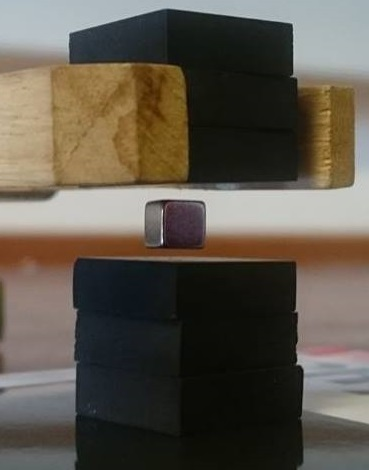
\includegraphics[width=0.28\textwidth]{floatingMagnet}
			\end{center}
			\vspace{-15pt}
			\caption{A neodymium magnet floating freely in diamagnetically
			stabilised levitation, unaffected by frictional forces}
		\end{wrapfigure}

		The team has chosen to incorporate a small, modular, experimental
		compartment in the cansat. It will be used to house a small diamagnetically
		stabilised levitating ferromagnet, from which, energy from the vibrations in 
		the cansat may be harvested through use of a tuned inductor coil positioned
		close to the levitation experiment. The aim is to propose an alternative to
		traditional space and aircraft power acquisition methods such as solar arrays
		providing an advantage as it is able to be deployed from launch and allows
		otherwise wasted energy from other modules to be added back into the
		system. As a caveat, this method goes largely untested and therefore the
		primary purpose of the team’s experimentation is to test if this is a viable
		alternative to traditional power sources.\\\\
\noindent
		{\color{blue}
		As a stretch goal, the team is now also looking to make several additional
		experimental modules, so that the ability to switch experiments may be 
		demonstrated, as well as possibly utilised for a physical launch. One of the 
		experiments currently being researched are researching use of two 
		Geiger--Muller tubes to measure changes in frequency of cosmic showers 
		and collisions.
		\\\\
		Another experiment that the team is considering is the use of infrared,
		visible light and other electromagnetic sensors to determine the health of
		vegetation, which can be applied to forests, plantations and nature conservation
		zones, in order to survey overall health of vegetation in these respective
		areas.
		\\
		}

		
		\begin{figure}[H]
			\begin{center}
				
\includegraphics[width=0.3\textwidth]{placeholder}
			\end{center}
			\vspace{-10pt}
			\caption{Proposed wireframe design of base station live processing graphs
			and parameter display}
		\end{figure}


		\subsection{What Will be Measured, Why and How}
		\begin{table}[H]
		\setlength{\tabcolsep}{6pt}
		\begin{tabularx}{\textwidth}{@{} YYY @{}}
        		\toprule
        		\textbf{What will be measured} & 
		       \textbf{Why is it being measured} & 
		       \textbf{How is it being measured}\\
		       \midrule
		
		       High fps camera footage. 
		       & Have a visual record of the secondary mission events. 
		       & Using the ArduCam OV5640 camera module.\\
		
		       \addlinespace
		       Barometric pressure, temperature, humidity and environmental gasses. 
		       & For telemetry to base station, fulfilling primary mission. 
		       & Via a PCB-integrated Bosch BME680.\\
		
		       \addlinespace
		       $V_{rms}$ across secondary mission inductor coils. 
		       & For power calculations and analysis from base station. 
		       & A MOSFET full-bridge rectifier converts AC to DC without voltage
			drop. A non-inverting amplifier is used to proportionally increase voltage
			output. A high resolution linear ADC reads voltage.\\
		
		       \addlinespace
		       GPS coordinates. 
		       & To aid cansat tracking. 
		       & The MTK3339 GPS is mounted to the main PCB and wired to a
			dedicated antenna on the side of the cansat.\\
		
		      \addlinespace
		      Rotation, acceleration and relative position. 
		      & Additional data to aid primary and secondary mission. 
		      & FXOS8700 + FXAS21002 9DOF module soldered to the main PCB.\\
		
		      \addlinespace
		      Vibrations. 
		      & Data for secondary mission power generation performance. 
		      & Accelerometer from 9DOF package.\\
	
		      \addlinespace
		      $I_{rms}$ generated by secondary mission inductor coils. 
		      & For power calculations and analysis from base station. 
		      & A MOSFET full-bridge rectifier converts AC to DC without voltage
			drop. An ACS712ELC in series with the inductor coil measures DC 
			current generated by the setup. \\
		     \bottomrule
		\end{tabularx}
		\end{table}
		\vspace{6pt}

		{\color{blue} \textbf{Changes Made}
		\begin{itemize}
			\item 3D magnetic field strength is a redundant feature to measure
			and will not provide relevant data to the secondary mission. Therefore,
			it has been removed from the cansat design to streamline space, 
			performance, etc.
			\item Vibrations will be more accurately measured using the 
			accelerometer onboard the cansat, hence, the mechanical vibration
			sensor has been removed due to redundancy.
			\item The bridgetek CleO-CAM1 camera module from the former 
			report was overly complex for this application, in addition to being
			difficult to interface with. This has since been changed to the ArduCam
			OV5640, which utilises the same optical sensor, but is able to interface
			via I$^2$C (so is easily interfacable), has lower power consumption, and
			is more compact.\\\\
		\end{itemize}
		}
		


\chapter{Cansat Description}
	\section{Overview}
		This year’s entry has taken much more of an emphasis on a scientific
		experimental module as the secondary mission. Hence, we have designed 
		the cansat with a focus on technical and scientific accuracy. We aim to
		complete most of the cansat construction in-house. The only part of the
		cansat that we anticipate outsourcing is the PCB for the cansat, as we do
		not have access to the materials or machinery for creating our own.
		\\\\
		Care was taken to ensure that the electronic sensors used are not 
		negligibly affected by strong and changing magnetic fields, however 
		testing will be required later to confirm that this is not an issue before 
		any launches.
		\\\\
		{\color{blue}Although our cansat must be technically very accurate to ensure
		a successful secondary mission, the team also values the cansat's ability
		to be able to switch out experimental modules with ease, meaning that
		other experiments can be conducted within quick succession and minimal
		effort.}

	\section{Mechanical Design}

		\begin{wrapfigure}{r}{0.34\textwidth}
			\vspace{-47pt}
	 		\begin{center}
			
\includegraphics[width=0.30\textwidth]{placeholder}
			\end{center}
			\vspace{-15pt}
			\caption[X]{Prototype frame for experimental module compartment}
		\end{wrapfigure}

		The cansat is designed with a modular secondary mission compartment. 
		This will allow the cansat to be used with different experimental apparatus 
		in the future. A rail system will allow experimental apparatus to be set up,
		then slid into place and secured. Any electrical connections can be easily
		made with our modified pin-headers that lead to I2C terminals, GPIO and
		other commonly accessed pins. The experimental module proposed for 
		our entry is held together with a 3D printed frame and assembled by 
		hand, with an adjustable height magnet.
		\\\\
		The main cansat assembly is also secured with a lightweight 3D printed
		internal frame, which allows reliable mounting and placement of components
		and wiring. It is surrounded by a hand-made fiberglass shell, which will flex
		upon impact serving to absorb and disperse much of the shock of the
		cansat landing or any other collisions. Plastic plates are used on the top and
		bottom of the cansat for further protection of the cansat from shock. The 
		$\frac{1}{2}\lambda$ dipole communications antenna is mounted outside
		the outer shell along the long axis in order to optimise communications.

		%Need to get a better photo - this one is low res, off-centre, 
		%pulled from google doc, etc.
		\begin{figure}[H]
			\begin{center}
				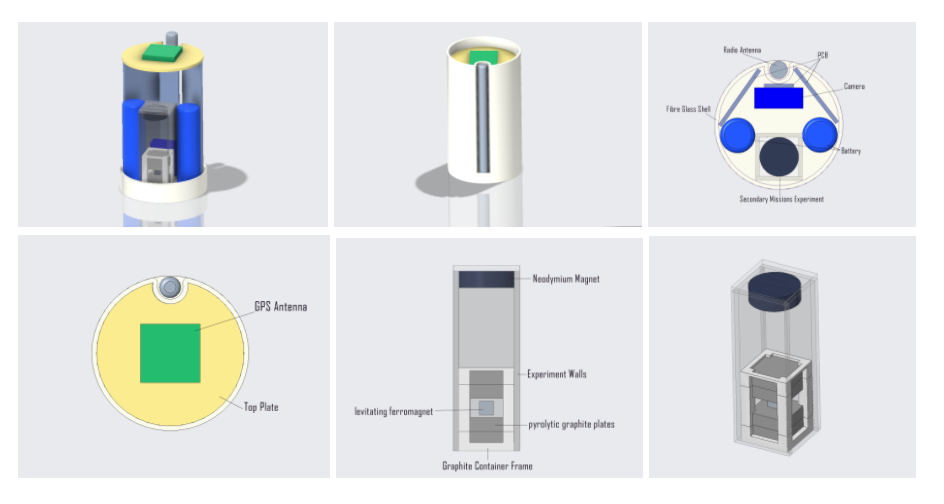
\includegraphics[width=0.8\textwidth]{CadRenders}
			\end{center}
			\vspace{-15pt}
			\caption{Computer--aided design (CAD) renders of the mechanical design}
		\end{figure}


	\section{Electronics Design}
		Two independent cells are symmetrically distributed in the cansat and
		connected in series to deliver native 3.7V DC power to the cansat at 
		4800mAh power to the cansat sub-systems.
		Built-in IPS (Intelligent Power Select) in the CHIP Pro enables management
		of the power delivered to the other sub-systems in the cansat, providing
		flexible control over the battery life of the cansat. 
		\\\\
		The inductor coil from the secondary mission outputs an AC current, which
		is converted to a DC rms current via full-bridge rectifier and the output
		current and voltage read by the industry-standard ACS712 and a 
		high--resolution ADC respectively, since the CHIP Pro built-in ADC 
		does not offer a satisfactory resolution for the experimental precision.
		\\\\
		{\color{blue}For interfacing purposes, an arduino pro mini has been
		implemented to the electronics design. This will be used as a hard interface
		between the CHIP Pro and select sensors, in addition to possibly providing
		regulated power to some parts of the system. The arduino will not be 
		executing any complex calculations or data aggregation.}
		
		\begin{figure}[H]
			\begin{center}
				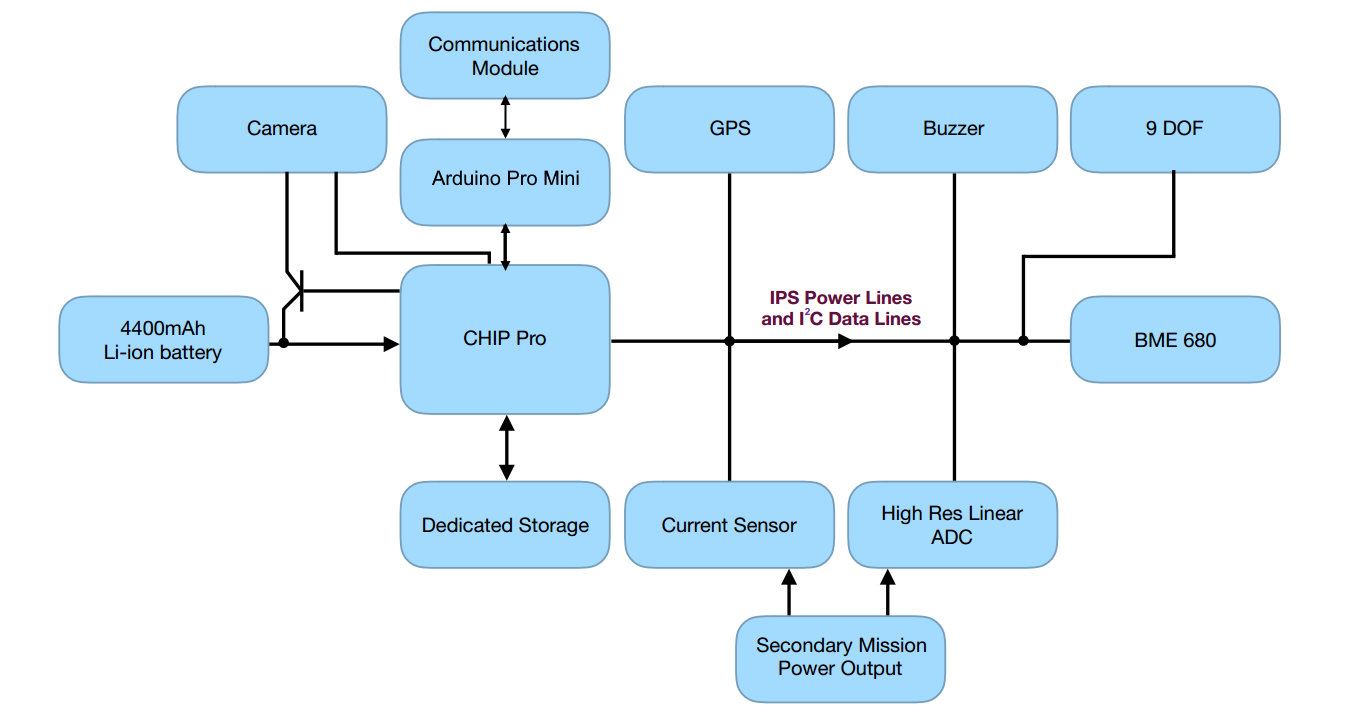
\includegraphics[width=0.7\textwidth]{electronics}
			\end{center}
			\vspace{-15pt}
			\caption{Electronics sub-systems diagram}
		\end{figure}


	\section{Software Design}

		\begin{wrapfigure}{r}{0.45\textwidth}
			\vspace{-30pt}
	 		\begin{center}
			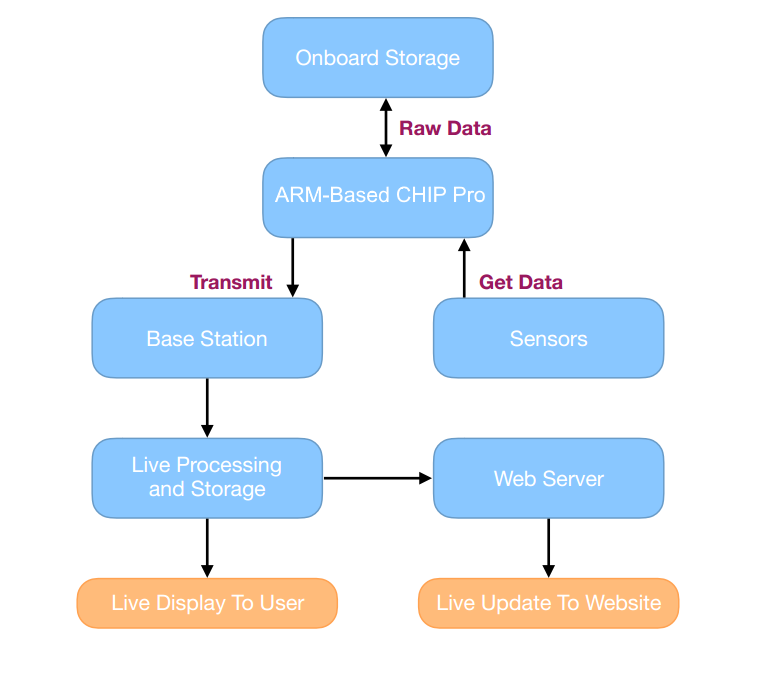
\includegraphics[width=0.45\textwidth]{software}
			\end{center}
			\vspace{-15pt}
			\caption[X]{Software system architecture diagram}
		\end{wrapfigure}

		The CHIP reads all incoming sensor data and applies lightweight processing
		to the values. All raw data is stored in built-in NAND storage on the CHIP
		or select raw data (larger sets such as camera footage) is stored in an
		onboard SD card for retrieval from ground crews. The processed data sets 
		are transmitted via 5 channels on a 433MHz frequency at up to 5,000bps
		baud rate. This allows for dedicated sensor channels in addition to a control
		channel, giving clean and organised telemetry of packets, as well as being
		able to pause telemetry of lower priority channels in cases of low 
		connection stability.
		\\\\
		The decision to use the CHIP Pro over a typical arduino or Raspberry Pi
		package was based on the 64--bit ARM--based processor running a 
		native Linux operating system, as well as built-in hardware to handle 
		wireless networking, bluetooth and battery regulation systems.
		\\\\
		{\color{blue}Previous iterations of the system architecture required 
		an Arduino Pro Mini in addition to the CHIP Pro for interfacing purposes.
		This year, the team aimed to omit this from the system requirements.
		Unfortunately, given the time and feasibility constraints, this must be deferred
		until later consideration.
		\\\\
		Additionally, the original plan to divide telemetry into
		5 channels may be less feasible than first envisaged. In which case, we will 
		take care to organise packets neatly on a lower number of bands.
		}

	\section{Landing and Recovery System}

		\begin{wrapfigure}{r}{0.45\textwidth}
			\vspace{-30pt}
	 		\begin{center}
			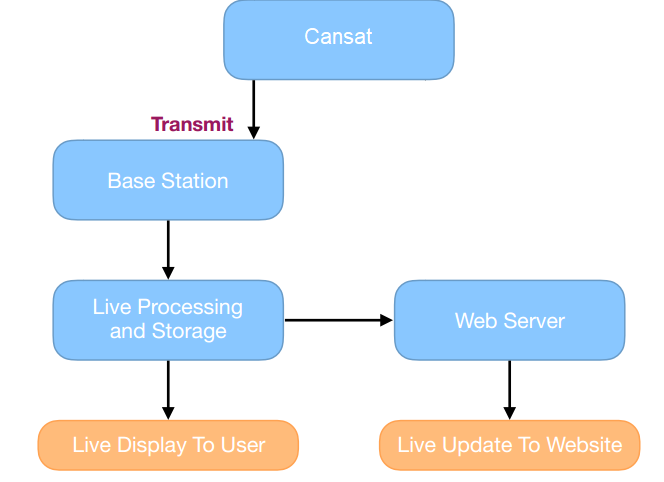
\includegraphics[width=0.45\textwidth]{ground}
			\end{center}
			\vspace{-15pt}
			\caption[X]{Landing and recovery system diagram}
		\end{wrapfigure}

		We plan to use a basic drag parachute design to regulate the cansat’s 
		descent speed. On landing, the fiberglass outer shell will flex, absorbing 
		some of the landing shock. Our cansat will have both a dedicated
		communications antenna and gps antenna. This means we will have 
		better connection to the base station and a high chance of accurate GPS lock,
		further assisting the recovery team in locating the cansat.
		\\\\
		{\color{blue}As an additional measure, foam padding will be added 
		directly underneath the batteries to protect them from extensive damage, which
		could otherwise risk the battery life of the cansat during the recovery phase of
		the launch.
		\\\\
		A buzzer will also be implemented to the design, which will sound
		after the cansat enters post-landing mode, which will sound at approximately
		90db, which is equatable to the amplitude of a jet from 300m distance.}

	\section{Ground Support Equipment}
		The team is developing a lightweight, robust base station program, which 
		can be executed with very low system requirements. This has inspired a
		stretch goal to create an all-in-one base station by setting up the base 
		station software on a Raspberry PI package, as well as the communications
		module and I/O for SMA, display outputs, and USB ports.
		\\\\
		Our base station equipment will include:
		\begin{itemize}
			\item Custom made base-station computer with WiFi and bluetooth
			connectivity and >3 USB ports.
			\item HC-12 communications module and dedicated Yagi antenna
			\item Battery charging station and 5V supply
		\end{itemize}
		Our base station will receive, aggregate and display live data
		from all the onboard sensors, showing the relevant graphs to our primary
		and secondary missions, respectively. It will also store all raw and 
		processed data locally, in addition to backing up to an external drive or 
		laptop.
	

\chapter{Project Planning}
	\section{Gantt Chart}
	\begin{figure}[h]
		\centering
		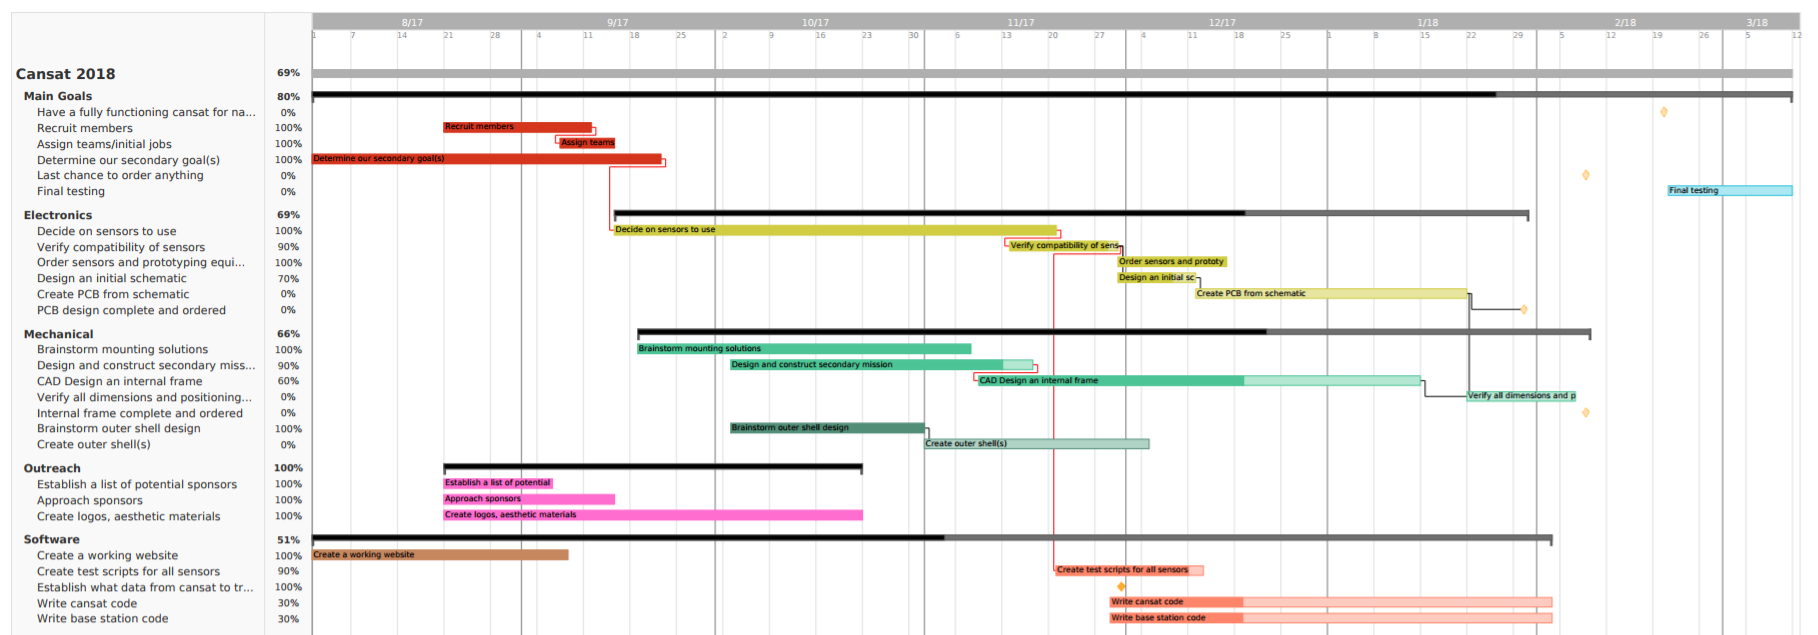
\includegraphics[width=\textwidth]{ganttDec.PNG}
		\caption{Gantt chart as of December 2017. Full resolution chart 
		available at:\url{https://goo.gl/dDAatf}}
	\end{figure}
	
	\section{Team and External Support}
		We currently have five team members with varying levels of experience in
		mechanical, electronic, and software design. While our team has a good
		technical background in all aspects required for cansat design, {\color{blue}
		We have now completed a training programme to ensure the team is 
		prepared for the competition with the appropriate skills.}
		\\\\
		We also continue to arrange occasional meetings and communications with
		professionals in various relevant industries, thus improving our 
		understanding of how to further improve the quality of our electronics 
		and mechanical design decisions, as well as aiding us in preparing our
		secondary mission.
	\clearpage
	\section{Risk Analysis}
		\begin{table}[h!]
		\setlength{\tabcolsep}{6pt}
		\begin{tabularx}{\textwidth}{@{} YY @{}}
			\toprule
			\textbf{Potential Issue} & 
			\textbf{Mitigation Method}\\
			\midrule
			Unable to produce fiberglass shell with required durability or tolerances. &
			Use 63mm PVC tubing instead of fiberglass. We already have a source 
			for the PVC tubing.\\
			\addlinespace
			Communications modules do not have required range with Yagi antenna.  
			& Use provided radio modules instead of HC-12 radio modules.\\
			\addlinespace
			Cansat does not meet battery life requirements. & 
			2 more cells will be implemented, giving 9600mAh of battery life 
			(double that of the current design).\\
			\addlinespace
			Cansat is over budget. &
			We will remove non-critical systems from the cansat or move to a 
			more conservative design based around the supplied kit.\\
			\addlinespace
			Cansat is overweight. &
			We will create an polymer internal frame to replace the 
			current aluminum design.\\
			\addlinespace
			Cansat is underweight. &
			We will add 2 more cells, serving to increase battery life in addition to
			solving weight issues. We also have space for ballast weight on the
			bottom of the cansat.\\
			\addlinespace
			Missing internal space necessary to implement all proposed sensors. &
			Select sensors will be removed to meet size spec.\\
			\addlinespace
			{\color{blue}
			Diamagnetically stabilised levitation experiment is not working as 
			intended} &
			{\color{blue}We are working towards creating multiple alternate
			experimental modules
			along with programs for them. This will also allow us to demonstrate the
			modular abilities of the cansat.}\\
			\addlinespace
			Magnetic fields interfering with electronics or communications. &
			Iron shielding will be placed between the experiment and electronics, 
			or around the experiment.\\
			\bottomrule
		\end{tabularx}
		\end{table}
		\clearpage
	\section{Test Plan}
		\begin{table}[h!]
		\setlength{\tabcolsep}{6pt}
		\begin{tabularx}{\textwidth}{@{} YY @{}}
			\toprule
			\textbf{Feature to Test} & 
			\textbf{Testing Method}\\
			\midrule
			Radio transmission. &
			Radio range and transmission tests will be conducted line-of-site in an
			open field with our final Yagi antenna, as well as forestry and a hill. We
			have already organised an ideal location for this.\\
			\addlinespace
			Cansat parachute. & 
			The cansat will be dropped from a drone at heights from 100 to 200
			meters in accordance with the cansat guidelines document.\\
			\addlinespace
			Power consumption and battery life. &
			Power consumption and battery life will be tested by measuring active
			battery life under a variety of temperature conditions.\\
			\addlinespace
			Cansat durability. &
			The cansat frame will be dropped, with electronics substituted with
			weights, from a variety of heights to simulate worst-case parachute
			conditions.\\
			\addlinespace
			Robustness of cansat and base station code. &
			All inputs and functions of the programs will be extensively tested to
			ensure that our software design will perform to a high standard.\\
			\addlinespace
			
			\bottomrule
		\end{tabularx}
		\end{table}

\chapter{Outreach Programme}
	\begin{wrapfigure}{r}{0.33\textwidth}
		\vspace{-60pt}
 		\begin{center}
		
\includegraphics[width=0.30\textwidth]{Logo}
		\end{center}
		\vspace{-15pt}
		\caption[X]{New Team Logo}
	\end{wrapfigure}

	In addition to the following, the team has also renewed the graphical designs
	for this campaign, which will help to give the team a fresh and stand--out
	aesthetic.
	
		
	\section{Media}
		For this years outreach we have designed, programmed and are hosting our
		own website at \url{gwccansat.com}.\\\\
		We also host pages on Instagram, Facebook and Twitter, giving regular
		updates	on our Team's progress.\\\\

		\begin{wrapfigure}{l}{0.37\textwidth}
			\vspace{-30pt}
	 		\begin{center}
			
\includegraphics[width=0.34\textwidth]{youtube}
			\end{center}
			\vspace{-15pt}
			\caption[X]{Team YouTube channel}
		\end{wrapfigure}

		\noindent
		The team's YouTube channel now has a fortnightly video blog, where we
		will be informing viewers of our progress. Several videos have already been
		released and we look forward to receiving feedback on this aspect of our
		project. Our channel can be viewed here: \url{https://goo.gl/YxHHkH} and 
		our first video can be viewed here: \url{https://youtu.be/tEawegQ2coM}\\\\\\
		We aim to livestream much of the development process, such 
		as the electronics PCB design and mechanical CAD modelling. Additionally, we
		would like to livestream and record elements of the competition experience
		this year, to show to our sponsors and other interested viewers, as we
		have received a magnitude of positive engagement and interest in this 
		aspect of the competition.
	
	\section{Physical Press}
		Following the success of our booth at the 2017 Edinburgh maker faire, we
		have signed up to attend as makers again this year. We are aiming to
		further improve our setup to engage interested parties (particularly children)
		in the 
		project to a greater extent than previously, including potential interactive
		programming or engineering challenges.\\\\
		\clearpage

		\begin{wrapfigure}{r}{0.35\textwidth}
			\vspace{-30pt}
	 		\begin{center}
			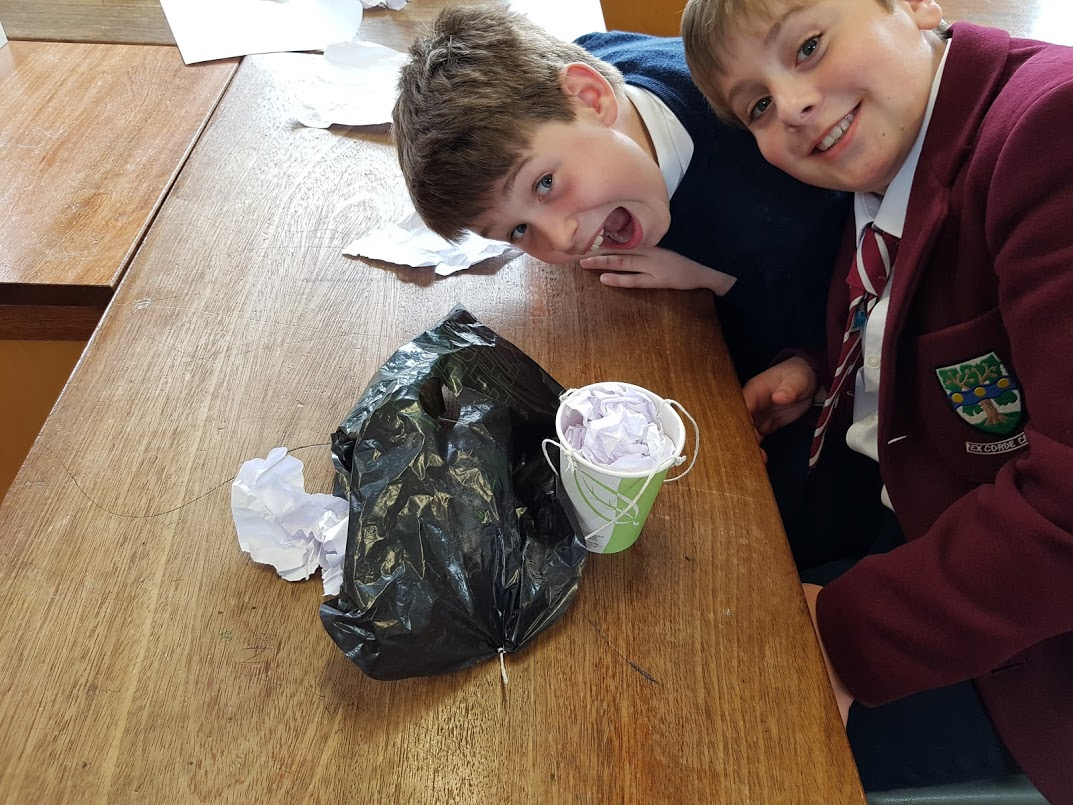
\includegraphics[width=0.31\textwidth]{p5s}
			\end{center}
			\vspace{-15pt}
			\caption[X]{Primary school children getting involved in parachute design}
		\end{wrapfigure}

		\noindent
		Additionally, we will continue to participate in engaging younger children
		from the GWC junior school with STEM education, as we did last year.
		We believe that in engaging kids with STEM at a young age, we will continue
		to inspire generations of scientists and engineers to come. We will also
		research into organising visits to other primary schools around the Edinburgh
		area.\\\\
		Following the largely successful 2017 campaign, the team featured in the
		 `Edinburgh Evening News' and aims to feature in other larger scale press
		releases such as this in future months.


\end{document}